\chapter{Die \glqq ideale\grqq{} Dev(Sec)Ops Pipeline}

Bereits im letzten Abschnitt wurde klar: Jeder kann sich Elemente der DevOps-Kultur aneignen und nach belieben kombinieren. 
Eine \glqq Musterlösung\grqq{} für den idealen Prozess kann es also nicht geben. 

Trotzdem gibt es Anordnungen der CI/CD/CT-Pipeline, die Vorteile gegenüber anderen Anordnungen mit sich bringen. 

In diesem Kapitel soll eine Pipeline beispielhaft modelliert und nach einer persönlichen Einschätzung hin optimiert werden.

\section{Welche Werkzeuge kommen zum Einsatz?}\label{sec:welchetools}

Die Zahl der CI/CD-Werkzeuge, die bei der Konstruktion einer Pipeline zur Verfügung stehen ist groß \cite{xebialabsXebiaLabsPrasentiertPeriodensystem2018} \cite{digital.aiPeriodicTableDevOps}. Würde man versuchen jedes Werkzeug zu integrieren / zu thematisieren, so könnte man keinem gerecht werden.
Aus diesem Grund soll an dieser Stelle eine Auswahl an Werkzeugen behandelt werden. Diese setzt sich zusammen aus den Werkzeugen die im Seminar behandelt wurden, Teil von Vorträgen waren oder vom Autor als wichtig erachtet werden.

Die folgenden Abschnitte bieten eine Übersicht über die betrachteten Werkzeuge. Dabei werden diese in die Kategorien CI/CT/CD eingeteilt. Es wird eine kurze Erklärung gegeben, was das Werkzeug bewirkt und mit welchem realen Produkt die Stufe besetzt werden könnte.

\subsection{Abschnitt: Continuous-Integration}
\begin{enumerate}[resume]
    \itemsep-0.5em 
    \item \textbf{Coding Style Guidelines}\label{Coding Style Guidelines} \\
        Überprüfung, ob die \emph{Coding-Conventions} eingehalten werden. Sollte direkt in der IDE des Entwicklers überprüft werden. Hierfür kann ein \emph{Linter} \cite{guimaraesWhatLinterWhy2020} zum Einsatz kommen. Welcher ist dabei von der Programmiersprache abhängig.
    \item \textbf{Code Architecture}\label{Code Architecture} \\
        Überprüfung, ob \emph{architekturelle Konventionen} und \emph{Namenskonventionen} eingehalten werden. Sollte direkt in der IDE des Entwicklers überprüft werden. In den Seminarvorträgen wurde hierfür das Werkzeug \emph{Arch Unit} \cite{gafertArchUnit} ausgewählt.
    \item \textbf{Commit-Conventions}\label{Commit-Conventions} \\
        Um die Einhaltung der \emph{Commit-Merge}-Konventionen garantieren zu können, sollten Regeln im Dependency-Manager gesetzt werden. GitHub und GitLab beispielsweise können so konfiguriert werden, dass Merges nur von bestimmten Branches den Produktions-Branch vorgenommen werden dürfen. Durch einfache Skripte kann auch das Format der Commit-Nachrichten überprüft werden \cite{ConventionalCommits}.
    \item \textbf{(Pre-) Versioning}\label{(Pre-) Versioning} \\
        In der Softwareentwicklung ist die Vergabe inkrementeller Versionsnummern für die bessere Übersichtlichkeit entscheidend \cite{preston-wernerSemanticVersioning}. In der Pipeline können für bestimmte Merges Versionsnummern entweder geprüft oder sogar automatisch vergeben werden. Mit kurzen Skripten kann auch ein automatisiertes \emph{Tagging} von Releases im Dependency-Manager vorgenommen werden.
    \item \textbf{License-Checker}\label{License-Checker} \\
        Um den korrekten Umgang mit (Open-Source)-Lizenzen frühzeitig zu unterstützen, können automatisierte Lizenz-Überprüfungen vorgenommen werden. Hierauf wird in \autoref{chapter:license-checker} genauer eingegangen.
\end{enumerate}

\subsection{Abschnitt: Continuous-Testing}
\begin{enumerate}[resume]
    \itemsep-0.5em 
    \item \textbf{Unit-Tests}\label{Unit-Tests} \\
        Die Grundlage eines Test-Frameworks wird von den sehr schnell ausführbaren \emph{Unit-Tests} gebildet. wie die Tests ausgeführt werden, ist von der Programmiersprache abhängig. Zum Einsatz kommen können beispielsweise \emph{jUnit} oder \emph{phpUnit}.
    \item \textbf{Vulnerability-Checker}\label{Vulnerability-Checker} \\
        Mithilfe dieses Werkzeuges können Schwachstellen oder Sicherheitslücken in Drittan\-bieter-Bibliotheken erkannt werden und die Kompatibilität von Abhängigkeiten kann gewährleistet werden. In den Seminarvorträgen wurde hierfür das Werkzeug der Plattform \emph{Snyk} eingesetzt \cite{snykOpenSourceSecurity}.
    \item \textbf{E2E-Tests}\label{E2E-Tests} \\
        Um die Funktionsweise einer vollständigen Anwendung in der Produktionsumgebung zu testen, kann ein sog. \emph{End-to-End Test} eingesetzt werden. 
        Im Bereich der Webentwicklung können hier beispielsweise \emph{Browsertests} mit dem Werkzeug \emph{Selenium} durchgeführt werden \cite{seleniumSeleniumAutomatesBrowsers}.
    \item \textbf{Dynamic Application Security Testing (DAST)}\label{DAST} \\
        Eine Vielzahl von Sicherheitslücken wird durch wiederkehrende Programmierfehler verursacht. Um dem vorzubeugen, kann nach häufigen Sicherheitslücken in einer Applikation automatisiert gesucht werden. In den Seminarvorträgen wurde hierfür das Werkzeug von GitLab eingesetzt \cite{gitlabDynamicApplicationSecurity}.
    \item \textbf{Application Security Management; Test/Code Coverage Statistiken}\label{Test/Code Coverage Statistiken} \\
        Um die Informationen aus Tests und anderen Quellen möglichst gezielt verwende zu können, sollten diese zentral aggregiert und einheitlich zusammengefasst werden. 
        Dieser Schritt dient mehr der Gesamtübersicht, anstatt neue Informationen zu gewinnen.
\end{enumerate}

\subsection{Abschnitt: Continuous-Delivery}
\begin{enumerate}[resume]
    \itemsep-0.5em 
    \item \textbf{Application Building}\label{Application Building} \\
        Automatisiertes Kompilieren von Packen von Code zu ausführbaren Dateien oder Anwendungen kann durch einfache Skripte in grundlegenden Pipelines vorgenommen werden. Besonders ist dabei, dass leicht für verschiedene Prozessorarchitekturen und Betriebssysteme kompiliert werden kann.
    \item \textbf{Application Deployment}\label{Application Deployment} \\
        Automatisches ausrollen das Code in die Produktionsumgebung wird von praktisch jedem Pipelinesystem nativ unterstützt. Sollte ein spezielles Vorgehen erwünscht sein, kann zusätzlich mit SSH und einfachen Skripten unterstützt werden. Fokus sollte auf der permanenten Erreichbarkeit der Produktionsumgebung liegen, was beispielsweise mit \emph{Zero Downtime Deployment} erreicht werden kann \cite{craftquestWhatAreZero}. 
    \item \textbf{Application Monitoring}\label{Application Monitoring} \\
        Um die kontinuierliche Verfügbarkeit der Produktionsumgebung zu garantieren und auf Anomalien reagieren zu können, sollte aktives \emph{Monitoring} verwendet werden. In den Seminarvorträgen wurde hierfür das Werkzeug \emph{Sentry} eingesetzt \cite{sentryApplicationMonitoringError}.
\end{enumerate}

\section{Wie ordnet man seine Pipeline am besten an?}

Nicht nur die Wahl der Werkzeuge ist entscheidend, sondern auch die Reihenfolge der Anordnung \cite{nemytchenkoGitLabCIRun2016}. 
Sinnvolle Priorisierung und Parallelisierung können die Feedback-Zeit verringern und die Server entlasten. 

Die Pipeline ist mit \emph{Integration}, \emph{Testing} und \emph{Delivery} in drei Hauptbestandteile zerlegt. Grafisch ist die Pipeline in \autoref{fig:cicdprocess} dargestellt. Die Nummerierung entspricht den entsprechenden Werkzeugen, die in \fullref{sec:welchetools} aufgelistet wurden.

Hauptziel dieser Pipeline ist, das Feedback möglichst zeitnah liefern zu können. Daher wurde versucht, die Werkzeuge möglichst so anzuordnen, dass die schnellen Tests und Überprüfungen zuerst liegen. \toolref{Coding Style Guidelines} kann praktisch in Echtzeit ausgeführt werden und liegt deswegen am Anfang des Prozesses. Der statische Check von \toolref{Code Architecture} kann ebenfalls in der IDE des Entwicklers ausgeführt werden. Bei großen Projekten sollte für diese Stufe auch ein Job in der Pipeline eingesetzt werden. \toolref{Commit-Conventions} und \toolref{(Pre-) Versioning} gehen mit jedem Commit in die Versionskontrolle einher. Damit die Qualität der Commits im weiteren Verlauf garantiert ist, werden diese zwei Schritte als erstes Element in der tatsächlichen Pipeline aufgeführt. 
\toolref{License-Checker} wird früh ausgeführt, da es sich um eine statische Analyse handelt, die schnell ausgeführt werden kann. Zudem können fehlerhafte Lizenzen den Gebrauch eines Paketes gänzlich unmöglich machen. Aus diesem Grund sollte diese rechtliche Überprüfung durchgeführt werden, bevor die \glqq teuren\grqq{} Testverfahren gestartet werden.

\begin{figure}[p]
    \vspace*{1cm}
    \setlength{\abovecaptionskip}{10pt}
    \setlength{\belowcaptionskip}{0pt}
    \centering
    \makebox[\textwidth][c]{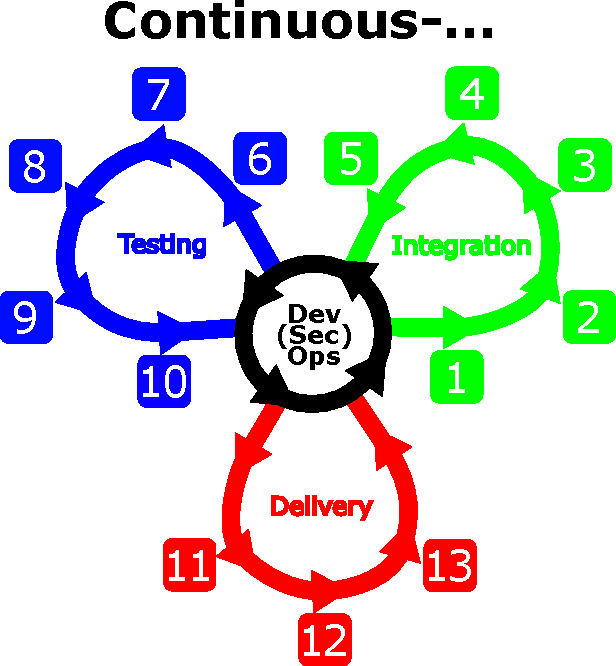
\includegraphics[width=\textwidth]{cicd_process.pdf}}
    \caption{Grafische Darstellung des \glqq idealen\grqq{} Dev(Sec)Ops Prozesses in Form einer CI/CT/CD-Pipeline. 
    Die drei Arme stellen die drei Phasen (Integration, Testing und Delivery) dar. Die Pfeile geben dabei die Richtung und den Weg an, in dem eine Änderung in die Produktionsumgebung über gehen kann. 
    Die Zahlen entsprechen dabei mit ihrer Nummerierung den Werkzeugen aus \ref{sec:welchetools}, wie sie in der Pipeline angeordnet werden. 
    Betont werden soll, dass über den inneren Kreis Stufen wiederholt werden können. Scheitert beispielsweise eine Änderung an einem Werkzeug in der \emph{Testing}-Phase, so wird die \emph{Delivery}-Phase innen übersprungen und mit der \emph{Integration}-Phase erneut begonnen. 
    Damit soll betont werden, dass Feedback von jedem Punkt schnell wieder zum Ausgangspunkt zurückfließen kann. }
    \label{fig:cicdprocess}
\end{figure}

Damit kann auch auf die makroskopische Funktionsweise der Pipeline nochmals eingegangen werden. Wie in \autoref{fig:cicdprocess} gut erkannt werden kann, wird die Pipeline in die drei Hauptäste \emph{Integration}, \emph{Testing} und \emph{Delivery} unterteilt. Durch den Verlauf der Pfeile wird klar, dass diese nacheinander durchlaufen werden müssen. Somit ist sichergestellt, dass der \emph{Testing}-Abschnitt nur nach erfolgreicher \emph{Integration} durchgeführt werden kann. Ebenso der \emph{Delivery}-Abschnitt nur nach erfolgreichen \emph{Tests}. Bei Fehlschlag eines Werkzeuges, ist jedoch immer der schwarze Weg zurück zum Anfang zu nehmen, um and den nicht ausgeführten Ästen vorbei zurück zum Start einer neuen Iteration zu gelangen. Dadurch ist die nacheinander Ausführung aufeinander aufbauender Test gewährleistet, und es müssen trotzdem (bei einem Fehlschlag) nur so wenige Schritte ausgeführt werden wie nötig.

Auch im \emph{Testing}-Abschnitt bauen die Tests von niedriger zu hoher Laufzeit und Komplexität aufeinander auf. Der Abschnitt beginnt mit \toolref{Unit-Tests}. Diese sind in den meisten Fällen noch schnell ausführbar ohne große Rechenleistung zu benötigen. Trotzdem decken sie bereits einen großen Teil der Funktionen eines Projektes ab. 
In der mittleren Phase des \emph{Testing}-Abschnittes kommt das erste Mal Parallelisierung zum Einsatz. \toolref{Vulnerability-Checker}, \toolref{E2E-Tests} und \toolref{DAST} arbeiten alle mit externen Pipelines oder vollständigen Versionen der Applikation. Tests auf diesen Umgebungen sind zumeist mit Wartezeiten oder der Nutzung höherer Rechenleistung verbunden. Dadurch können diese Abschnitte mehr Zeit in Anspruch nehmen als alle vorhergegangenen Werkzeuge. Daher bietet sich hier sehr gut an, diese \glqq teuren\grqq{} Tests erst hier und möglichst parallel auszuführen um weniger häufig lange auf das Ergebnis warten zu müssen.
\toolref{Test/Code Coverage Statistiken} schließt diesen Abschnitt ab. Da hier die Informationen aus den vorherigen Tests aggregiert werden, kann dieses Werkzeug nur hier platziert werden.

Nur eine vollständig getestete Applikation kann in den \emph{Delivery}-Abschnitt vordringen. Die Reihenfolge innerhalb dieser Stufe ist logisch vorgegeben. Zuerst muss der Code mit \toolref{Application Building} kompiliert und gepackt werden, damit die daraus resultierende Anwendung mit \toolref{Application Deployment} in die Produktionsumgebung übergeben werden kann. Diese aktive Umgebung kann im letzten Schritt mit \toolref{Application Monitoring} überwacht werden. Von dieser Stufe ist auch der Weg zur Integration am kürzesten, um im Fehlerfall mit direkt mit einer neuen Entwicklungs-Iteration beginnen zu können.

Zusammenfassend lässt sich diese Pipeline als \glqq ideal\grqq{} Bezeichnen, wenn das Ziel ist, einen Fehlschlag immer möglichst früh abzufangen. Damit wirken sich die Wartezeiten in den späteren Stufen seltener auf den Programmierer aus und es können möglichst viele der Probleme über die billigen Teststufen abgefangen werden.
Dies stellt nach der Meinung des Autors die effizienteste Nutzung der Ressourcen Zeit und Rechenleistung dar und ist daher anderen Formen der Ausführung überlegen.
